%%%%%%%%%%%%%%%%%%%%%%%%%%%%%%%%%%%%%%%%%
% University Assignment Title Page 
% LaTeX Template
% Version 1.0 (27/12/12)
%
% This template has been downloaded from:
% http://www.LaTeXTemplates.com
%
% Original author:
% WikiBooks (http://en.wikibooks.org/wiki/LaTeX/Title_Creation)
%
% License:
% CC BY-NC-SA 3.0 (http://creativecommons.org/licenses/by-nc-sa/3.0/)
% 
% Instructions for using this template:
% This title page is capable of being compiled as is. This is not useful for 
% including it in another document. To do this, you have two options: 
%
% 1) Copy/paste everything between \begin{document} and \end{document} 
% starting at \begin{titlepage} and paste this into another LaTeX file where you 
% want your title page.
% OR
% 2) Remove everything outside the \begin{titlepage} and \end{titlepage} and 
% move this file to the same directory as the LaTeX file you wish to add it to. 
% Then add \input{./title_page_1.tex} to your LaTeX file where you want your
% title page.
%
%%%%%%%%%%%%%%%%%%%%%%%%%%%%%%%%%%%%%%%%%
%\title{Title page with logo}
%----------------------------------------------------------------------------------------
%	PACKAGES AND OTHER DOCUMENT CONFIGURATIONS
%----------------------------------------------------------------------------------------

\documentclass[10pt, a4paper]{article}
\usepackage[a4paper,left=2cm,right=2cm,top=2.5cm,bottom=2.5cm]{geometry}
\usepackage[english]{babel}
\usepackage[utf8x]{inputenc}
\usepackage{amsmath}
\usepackage{graphicx}
\usepackage[colorinlistoftodos]{todonotes}

\begin{document}

\begin{titlepage}

\newcommand{\HRule}{\rule{\linewidth}{0.5mm}} % Defines a new command for the horizontal lines, change thickness here

\center % Center everything on the page
 
%----------------------------------------------------------------------------------------
%	HEADING SECTIONS
%----------------------------------------------------------------------------------------

\textsc{\LARGE Università degli studi di Milano-Bicocca}\\[1cm] % Name of your university/college
\textsc{\Large Data Science Lab for Smart Cities}\\[0.3cm] % Major heading such as course name
\textsc{\large Final Essay}\\[0.1cm] % Minor heading such as course title

%----------------------------------------------------------------------------------------
%	TITLE SECTION
%----------------------------------------------------------------------------------------

\HRule \\[0.4cm]
%{ \LARGE \bfseries Beyond Food Delivery, eCommerce and Food Retail Chains}\\[0.3cm] % Title of your document

%{ \LARGE \bfseries How to Renovate Small Grocery Stores and Why}\\[0.3cm] % 
{ \LARGE \bfseries How to Change our Food Shopping Habits and Why}\\[0.3cm] % 

{ \Large \bfseries The Case of Milan}\\[0.1cm] % Title of your document
\HRule \\[1.5cm]
 
%----------------------------------------------------------------------------------------
%	AUTHOR SECTION
%----------------------------------------------------------------------------------------

\large
\emph{Authors:}\\
Marco Scatassi - 883823- m.scatassi@campus.unimib.it \\   % Your name
Silvia Grosso - 881993- s.grosso9@campus.unimib.it   \\[1cm] % Your name

% If you don't want a supervisor, uncomment the two lines below and remove the section above
%\Large \emph{Author:}\\
%John \textsc{Smith}\\[3cm] % Your name

%----------------------------------------------------------------------------------------
%	DATE SECTION
%----------------------------------------------------------------------------------------

{\large \today}\\[2cm] % Date, change the \today to a set date if you want to be precise

%----------------------------------------------------------------------------------------
%	LOGO SECTION
%----------------------------------------------------------------------------------------


\includegraphics{figs/logo.png}\\[1cm] % Include a department/university logo - this will require the graphicx package
 
%----------------------------------------------------------------------------------------

\vfill % Fill the rest of the page with whitespace

\end{titlepage}


\begin{abstract}

  Food shopping habits are changing and the Covid pandemic has further consolidated these shifts, especially in urban areas. There is a preference for a new type of shopping that is fast and convenient. However, this approach transforms the logistics and transportation of food commerce and weakens social relationships. Above all, this change requires a renewal of policies against food waste that makes the individual citizen aware and an active participant. Firstly, this report aims to highlight the negative effects of new food shopping habits and evaluate the phenomenon using appropriate indicators. Additionally, we focus on the specific scenario of Milan, analyzing the distribution of various types of food shops in relation to area and population. Finally we propose an optimization model based on our data that provides, starting from a given point, the shortest path to nearby grocery shops. Our goal is to encourage the citizen to go shopping on foot and actively participate in the fight against food waste, encouraging the purchase of any unsold surplus food from each shop.      


\end{abstract}

\section*{Introduction}

In 1957 the first italian supermarket was born in Milan, a large ``American-style" shop that revolutionized the way of shopping. The concept of big shopping was born: shopping that lasts longer, done independently, no longer based on the trust of the retailer but on the brand of the products.
In 2011, the first food delivery platform, Just Eat, arrives in Italy. In these same years, e-commerce is also developing in the Food \& Grocery sector. Incentivised by the Covid-19 pandemic, food e-commerce is now an increasingly important part of the investments of food companies in our country. Shopping habits are transformed once again, in search of a faster and easier way for an increasingly more sedentary and loner customer. However, on the other hand, small groceries are in great difficulty, the relationship between customer and seller has almost disappeared and in addition, the customer is inclined to prefer a sedentary and unhealthy way of shopping. 
Beyond all the problems mentioned above, the crucial issue at the moment is the fight against food waste. The 2023 Waste Watcher survey on food waste reveals that more than 4 million tonnes of food were wasted in the italian supply chain in 2022, equivalent to an economic loss of more than 9 billion euro \cite{food_waste}.

\noindent The main objective of our project is to analyze in detail the current scenario in Italy and in particular in the area of Milan, evaluating the possible negative consequences of new food purchasing behavior and finally proposing a feasible solution.
In the first part of the report, we will introduce the main statistics related to the food shopping in Italy and in Milan, highlighting from our point of view the negative aspects of food shopping routines. In this regard, we will use certain indicators to measure the impact, be it social or individual, economic or ethical, of the problem we observe.
In the second part of the report, we will present the data we have collected on food shops in the municipality of Milan by using OpenStreetMap API and Places API by Google Maps Platform (citare url api?). We will analyze the data through appropriate visualizations and statistics.
Finally, we will suggest an optimization model developed to reroute food shopping habits towards a healthier, sustainable and more aware way of purchasing.

\section{Problem Description and Indicators}
%\subsection{The Crisis of Small Food Shops}
\subsection{New Food Shopping Habits: an Evidence-based Analysis}

The way of shopping has inevitably evolved. The rhythm of life has changed drastically, needs have changed. It is no longer the practice to go in the morning to buy freshly baked bread from the favourite baker of the neighbourhood. No longer do we go into shops and ask for ``the same as usual, thank you". Today it is our apps that remember our preferences. Or at most we wander around the supermarket looking for our favourite product, which they may have moved to another shelf. From the advent of supermarkets to today, shopping has changed in social relations, timing, product quality, product packaging. The transformation that was already underway, with the arrival of the Covid pandemic, quickly and inevitably adapted to new needs. If until the early 2020s, people regularly left their homes to shop in supermarkets and small shops, with the outbreak of the pandemic and the ban on unnecessary travel, many bought online for the first time. This need has put small grocery shops to a hard test. During the lockdown, the only way for the small retailer to maintain a connection with its customers was to deliver its products directly to their homes or to favour the so-called ``Click \& Collect". This is how the ``e-commerce of proximity" was born \cite{prox_ecom}. Nevertheless, this new frontier remains trendy even now despite the fact that fortunately there is no longer a health emergency. Customers have no intention of giving up the many new benefits they have achieved. According to a recent Netcomm study, Food \& Grocery in Italy alone grew by +8.8\% in 2022. In Europe, Italy tops the list with a 42\% penetration of food e-commerce (https://www.digitelematica.it/le-tendenze-2023-nel-foodgrocery-in-italia/). 

It must be noted, however, that this scenario inevitably creates strong disparities, depending on the age of the users, who are more or less familiar with digital technology, or depending on the proximity of their neighbourhood to the city.
Furthermore, it has to be said that the new trend of online shopping is not yet optimised at all. Delivery workers have to make deliveries as fast as possible, threatened by the negative consequences of a failed delivery, with means of transport that are not yet energy efficient and labor rights still appallingly poor. Moreover deliveries often have real-time tracking, to estimate and optimize travel as much as possible, with possible consequences on customer privacy.

\subsection{The Food Waste Generation Problem}

As previously mentioned, one of the main focuses of this report is the problem of food waste.
It is clear that with these drastic changes in food spending habits, policies against food waste need to be revolutionised in parallel.
Specifically, the city of Milan is particularly active on environmental sustainability policies.
Since Expo 2015, Milan approved the ``Milan Urban Food Policy Pact", an international pact on sustainable food policies with a strict five-year action plan. Ensuring healthy food for all, fighting food waste and poverty, promoting urban horticulture, and better managing water resources: these are some of the priorities that Milan has set for itself in its city food policy by networking among the various local administrations and providing concrete tools for action. The figure \ref{fig: policy} shows extracts from the framework of action in the minutes of the Milan City Council's deliberation.

\begin{figure}[h!]
  \centering
  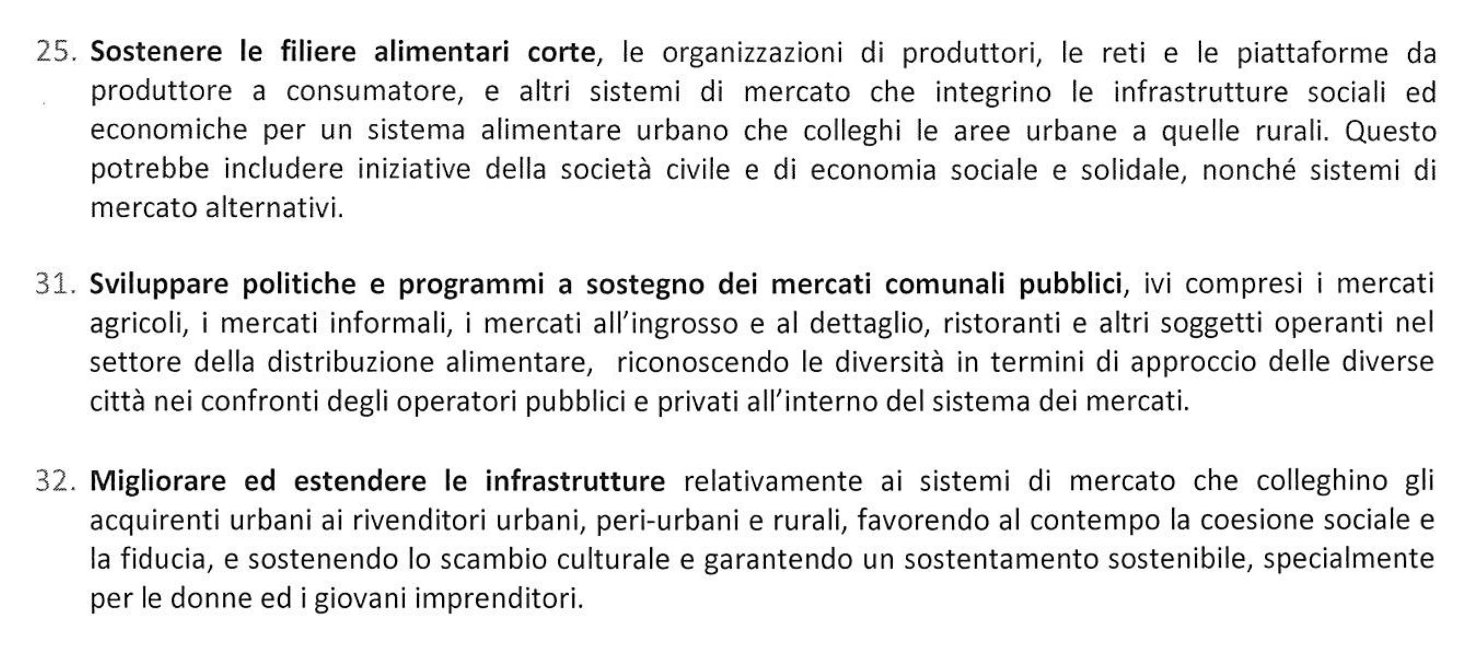
\includegraphics[width=14cm]{figs/food policy.png}
  \caption{Milan Urban Food Policy Pact: Suggested Actions}
  \label{fig: policy}
\end{figure}

We can notice a strong commitment to fostering social cohesion and maintaining a relationship of trust between the various stakeholders, while still ensuring a sustainable approach. We can summarize Food Policy priorities into five main points:

\begin{itemize}
\item ensure access to healthy food for all;
\item promoting the sustainability of the food system;
\item educating people on food;
\item fighting waste;
\item supporting and promoting local agri-food research.
\end{itemize}

Within the context of the \textit{Milan Urban Food Policy Pact}, in 2016, the Municipality of Milan, Assolombarda and the Milan Polytechnic shared the ``Zero Sprechi" protocol of intent with the aim of reducing food waste and innovating the methods for recovering food to be given to the needy, by designing and testing a model for recovering and redistributing food surpluses based on local neighbourhood networks. The actions started in 2018/2019 with the launch of an initial pilot project in City Hall 9. Today, as shown in the figure \ref{fig: hubs}, 5 neighbourhood Hubs are active for food recovery. The logistical model provides two daily recovery routes, morning and afternoon, allowing unsold or leftover food to be recovered and supplied to 21 target charities  (cita https://foodpolicymilano.org/hub-quartiere-spreco-alimentare/). 

\begin{figure}[h!]
  \centering
  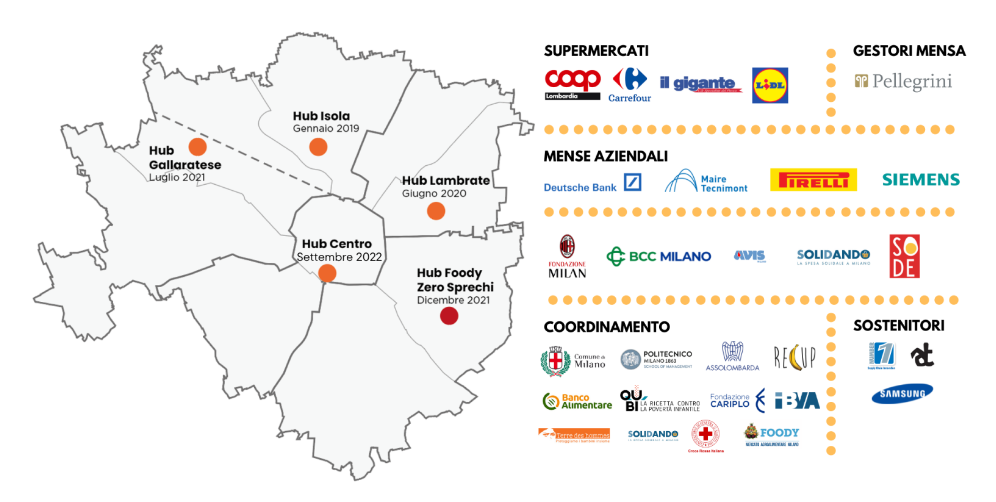
\includegraphics[width=9cm]{figs/hubs.png}
  \caption{Hubs in Milan (September 2022)}
  \label{fig: hubs}
\end{figure}

Although Milan is therefore strongly active in the fight against food waste, it can be seen that the policies currently active do not make responsible and directly involved the individual citizen. Furthermore, the supermarkets involved in the logistical model of neighbourhood Hubs do not gain direct economic benefit but only a reduction in taxes and a quality mark. Intoduce a strategy to involve directly local shops and citizens in the process could bring several benefits. If a policy of combating food waste with local shops and active participating citizens were developed in parallel, individual awareness would increase, the feeling of social cohesion would grow and small food businesses would gain a stronger identity again.

(presentare già qua la nostra idea?)

\subsection{The Need to Walk}

A further point we feel is important to examine is the impact of new spending habits on the health of the individual citizen. 
It is often considered a benefit to be able to do things directly from home. Nowadays, it is possible to work, enjoy a restaurant dinner, and even shop for groceries online, all from the comfort of our homes. However, besides the significant mental impact of these new habits, we must not overlook the risk of making our lives too sedentary with these practices.
Numerous studies demonstrate the importance and health benefits of incorporating movement throughout the day, even if it's relatively minimal and regardless of walking speed. The advantages in terms of mortality risk are highly evident. A recent meta-analysis involving 50000 individuals from four different continents shows that even as few as 6000 to 8000 steps per day for older adults and 8000 to 10000 steps for young adults can improve an individual's health and longevity(cita https://sph.unc.edu/sph-news/how-many-steps-lead-to-longevity-study-identifies-new-daily-goals/). It's evident that in the context of large cities, this theme is strictly related to the walkability in the urban space, i.e. the accessibility of amenities by foot. We recall here the definition of \textit{15-Minute City} model:

\begin{center}
\textit{``Cities should be designed so that, within a walking or cycling distance of 15 min from their residence, citizens should be able to meet all their daily needs: work, home, food, health, education, culture, sports, and leisure. 
''}
\end{center}

A recent study on walkability in Milan shows that, although the city has a strong potential to comply with the model of 15-Minutes City, there is still a challenge in the supply-demand mismatch (citare (https://transformtransport.org/research/livable-streets/walkability-and-the-15-minute-city-model-an-integrated-approach-for-the-city-of-milan/)). The population tends to live more in the suburbs while workers and services are concentrated in the city centre.
A sustainable growth of the city that is projected towards a more cycle-pedestrian mobility, must therefore guarantee a more granular and homogeneous network of food shops from the center to the suburbs and finally must spread individual well-being habits.

\subsection{The Impact on the City of Milan and its Inhabitants: some Possible Indicators}

We want to summarize in a clear and detailed manner some negative aspects that we have previously discussed regarding the transformation of our food shopping habits. We will use a set of indicators that will allow us to assess the economic, political, environmental, and social impact, both on the population and citizens, as well as on the city itself. These indicators will help us measure the problem clearly and evaluate our proposed solution.

    \begin{figure}[h!]
        \centering
        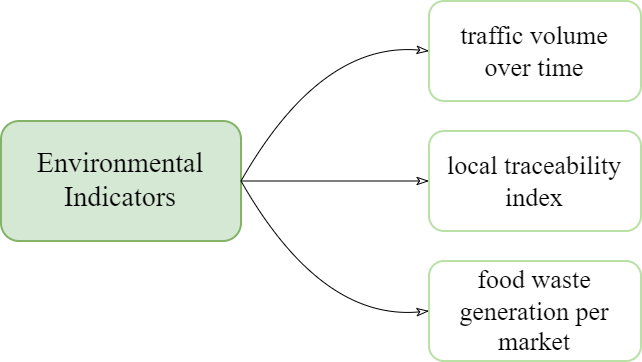
\includegraphics[width=7cm]{figs/env}
        \label{fig:env}
      \end{figure}
    

    % -more cars and traffic (traffic volume over time)
    % -more delivery not optimized -> https://www.ilsole24ore.com/art/food-delivery-big-contro-consegne-domicilio-troppo-inquinanti-AEITyJjC
    % -(food waste generation per market)
 
    \begin{figure}[h!]
        \centering
        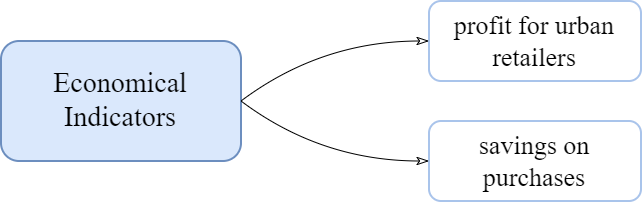
\includegraphics[width=7cm]{figs/econ}
        \label{fig:env}
      \end{figure}

    % economical
    % -crisis small shops owners 

    \begin{figure}[h!]
        \centering
        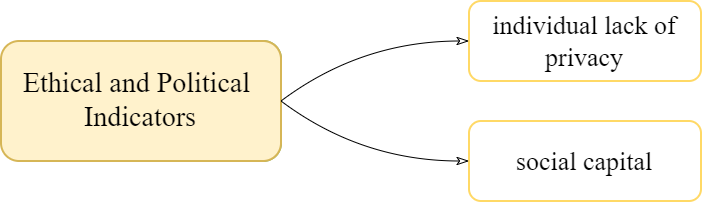
\includegraphics[width=7cm]{figs/health}
        \label{fig:env}
      \end{figure}

    % salute e benessere
    %     -sedentarity
    %     -stress (health and wellbeing Indicators)
    %     -solitude no more socialization -unawareness  (social capital)

    \begin{figure}[h!]
        \centering
        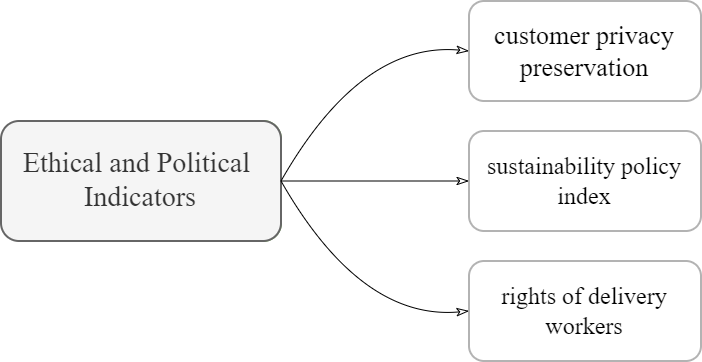
\includegraphics[width=7cm]{figs/ethic}
        \label{fig:env}
      \end{figure}

    % ethical and political
    %     -lack of privacy
    %     - ricerca equità nonostante differenze aree urbane / age gap / econimical gap





\newpage
\section{Data Analytics, Optimization and Policy Suggestions}

\subsection{Data Overview}

\subsection{Data Preparation}

\subsection{Data Visualization and Analysis}

\subsection{Addressing the Problem: an Optimization Model}

\subsection{Analysis of Optimization results}

\section*{Conclusions}

REM: 
An app that would show the citizen, considering my shopping list, a feasible walking distance in a few minutes between several shops might be a preferable choice for some who today perhaps rely on other solutions just because they are more practical.

\newpage

\bibliographystyle{IEEEtran}
\bibliography{references.bib}

\end{document}